\documentclass[11pt,a4paper,oneside]{article}

% -------------------------------------------------
% Basic packages
% -------------------------------------------------
\usepackage[T1]{fontenc}
\usepackage[utf8]{inputenc}
\usepackage[spanish,es-noquoting,es-nodecimaldot]{babel}
\usepackage{lmodern}
\usepackage{microtype}
\usepackage[a4paper,margin=1.18in,headheight=15pt]{geometry}
\usepackage{amsmath,amssymb,amsfonts,amsthm,mathtools}
\usepackage{bm}
\usepackage{enumitem}
\usepackage{booktabs}
\usepackage{array}
\usepackage{xcolor}
\usepackage{graphicx}
\usepackage{caption}
\usepackage{hyperref}
\usepackage{setspace}
\usepackage{fancyhdr}
\usepackage{titlesec}
\usepackage[most]{tcolorbox}
\usepackage{placeins}
\usepackage[capitalize,noabbrev]{cleveref}
\crefname{figure}{figura}{figuras}
\Crefname{figure}{Figura}{Figuras}
\crefname{section}{sección}{secciones}
\Crefname{section}{Sección}{Secciones}
\crefname{equation}{ecuación}{ecuaciones}
\Crefname{equation}{Ecuación}{Ecuaciones}

\hypersetup{
  colorlinks=true,
  linkcolor=blue!50!black,
  citecolor=red!55!black,
  urlcolor=teal!60!black,
  pdftitle={Sistema Integrado de Análisis Multirresolución y Desempeño Académico},
  pdfauthor={César Galindo López y Gabriel Villafuerte C.}
}

\theoremstyle{definition}
\newtheorem{definition}{Definición}[section]
\newtheorem{remark}[definition]{Observación}

\definecolor{ihesblue}{RGB}{25,62,114}
\definecolor{ihesgold}{RGB}{160,120,40}
\pagestyle{fancy}
\fancyhf{}
\fancyhead[L]{\textsc{Sentimiento por wavelet}}
\fancyhead[R]{\textsc{Galindo López \& Villafuerte C.}}
\fancyfoot[C]{\thepage}
\renewcommand{\headrulewidth}{0.35pt}
\renewcommand{\footrulewidth}{0pt}
\titleformat{\section}{\Large\bfseries\color{ihesblue}}{\thesection.}{0.65em}{}
\titleformat{\subsection}{\large\bfseries\color{ihesblue}}{\thesubsection.}{0.65em}{}
\titlespacing*{\section}{0pt}{1.9em}{1.05em}
\titlespacing*{\subsection}{0pt}{1.45em}{0.95em}
\tcbset{colback=white,colframe=ihesblue!65!black,boxrule=0.5pt,arc=1.5pt}
\setlength{\parskip}{0.85em}
\setstretch{1.13}
\setlength{\parindent}{0pt}
\captionsetup{font=small,labelfont=bf,labelsep=period}

\newtcolorbox{ideaBox}[1][]{enhanced,breakable,colback=blue!2,colframe=ihesblue,
  borderline west={1.5pt}{0pt}{ihesblue},title=Idea central,fonttitle=\bfseries,#1}
\newtcolorbox{summaryBox}[1][]{enhanced,breakable,colback=gray!4,colframe=black!55,
  borderline west={1.5pt}{0pt}{black!70},title=Fórmulas clave,fonttitle=\bfseries,#1}
\newtcolorbox{warningBox}[1][]{enhanced,breakable,colback=red!2,colframe=red!55!black,
  borderline west={1.5pt}{0pt}{red!75!black},title=Alcance y limitaciones,fonttitle=\bfseries,#1}
\newtcolorbox{implBox}[1][]{enhanced,breakable,
  colback=violet!3!white,colframe=violet!50!black,
  borderline west={2pt}{0pt}{violet!65!black},
  title=Implementación,fonttitle=\bfseries\color{violet!80!black},
  attach boxed title to top left={yshift=-2mm,xshift=4mm},
  boxed title style={colback=violet!12,colframe=violet!50!black,boxrule=0.5pt},#1}

\title{\vspace{-1.5cm}\textbf{\Large Sistema Integrado de Análisis Multirresolución y Desempeño Académico}\\[2pt]
\large Un índice de sentimiento con verificación estadística explícita de su eficiencia —y de sus límites—, vía embeddings y transformada wavelet}
\author{César Galindo López \\ \small Universidad Panamericana \textperiodcentered\ Facultad de Empresariales, Ciudad UP
  \and Gabriel Villafuerte C. \\ \small \href{https://github.com/Gabriel44svg}{github.com/Gabriel44svg}}
\date{\small 2026}

\begin{document}
\maketitle

\begin{abstract}
\noindent Presentamos un sistema que combina la señal cuantitativa de un curso (calificaciones,
parciales, estado de riesgo) con la señal cualitativa de una encuesta de retroalimentación
abierta, produciendo para esta última un índice de sentimiento por alumno
$\hat\theta\in(-1,1)$: cada respuesta se convierte en una señal escalar indexada por posición de
token (proyectando el embedding contextual de cada palabra sobre el embedding de oración), que
se descompone con la transformada discreta de onduleta (DWT) en un componente de tendencia
global y uno de fluctuación local. Acompañamos $\hat\theta$ de una verificación estadística
explícita —información de Fisher y cota de Cramér--Rao bajo los modelos gaussiano y
Laplaciano— y mostramos, con simulaciones, exactamente qué certifica esa verificación y qué no.
No reportamos corridas sobre datos reales de curso: este es un artículo de método,
acompañado de simulaciones ilustrativas explícitamente etiquetadas como tales, no un estudio de
caso.

\medskip
\noindent\textbf{Palabras clave:} analítica académica, alerta temprana, análisis de sentimiento,
transformada wavelet, información de Fisher, cota de Cramér--Rao.
\end{abstract}

\section{Introducción}

Un curso genera dos tipos de señal sobre el desempeño de un alumno: una \emph{cuantitativa}
(calificaciones parciales, tareas, exposición) y una \emph{cualitativa} (lo que el alumno
escribe en una encuesta de retroalimentación abierta). La señal cuantitativa es la que
normalmente se usa para detectar riesgo académico; la cualitativa suele leerse de forma
impresionista, sin métrica. Este trabajo propone una métrica para la segunda señal y pregunta si
aporta información adicional sobre el riesgo académico, vía su correlación empírica con la
calificación final.

La construcción de $\hat\theta$ combina dos ingredientes bien establecidos por separado:
\emph{embeddings} contextuales de oración obtenidos con redes tipo Siamese-BERT
\cite{ReimersGurevych2019}, y la transformada discreta de onduleta como herramienta de análisis
multirresolución de señales \cite{Mallat1989}. Lo que el sistema añade es una capa de validación
estadística explícita del estimador de sentimiento agregado del grupo, apoyada en la teoría
clásica de eficiencia de estimadores \cite{Fisher1922,Rao1945,Cramer1946}, complementada con una
prueba de normalidad \cite{ShapiroWilk1965} y una estimación de varianza por remuestreo
\cite{Efron1979}. La contribución de este artículo no es ninguno de esos ingredientes por
separado, sino documentar con precisión qué certifica —y, sobre todo, qué \emph{no} certifica—
su combinación, algo que la primera versión de nuestra propia implementación afirmaba de forma
imprecisa (\cref{sec:crb}).

\section{Arquitectura del sistema}

El sistema se organiza en cuatro módulos:

\begin{enumerate}[leftmargin=1.4em]
  \item \textbf{Ingesta y normalización} (\texttt{datos.py}): lectura de archivos de
  calificaciones (CSV/Excel) con detección automática de columnas (número de cuenta, nombre,
  parciales \texttt{E1,E2,\dots}, examen ponderado, tareas, exposición, validación), manejo de
  texto mixto en celdas no numéricas (\emph{``te presentas a final''}, \emph{``está en
  reposición''}, \emph{``baja''}, etc.) y cómputo de una bandera binaria de riesgo.
  \item \textbf{NLP y extracción wavelet} (\texttt{nlp\_wavelet.py}): embeddings de oración y de
  token (\emph{sentence-transformers} multilingüe) sobre las respuestas abiertas de la encuesta,
  y descomposición multirresolución de la señal posicional resultante vía DWT.
  \item \textbf{Validación teórica} (\texttt{cramer\_rao.py}): información de Fisher y cota de
  Cramér--Rao para el índice de sentimiento agregado, bajo los modelos gaussiano y Laplaciano,
  más prueba de normalidad (Shapiro--Wilk) y estimación bootstrap de la varianza del estimador.
  \item \textbf{Visualización interactiva}: interfaz Streamlit con páginas para carga de datos,
  métricas del curso, análisis de sentimiento y validación teórica, con interpretaciones
  automáticas en lenguaje natural para cada métrica.
\end{enumerate}

\section{Métodos}

\subsection{Bandera de riesgo académico}

Sea $c_i$ la calificación final del alumno $i$ y $e_i\in\{\text{Normal},\ldots\}$ su estado de
validación (reposición, examen final, baja, etc.). El sistema define
\[
r_i = \mathbf{1}\{c_i < 70\} \ \vee\ \mathbf{1}\{e_i \neq \text{Normal}\},
\]
es decir, un alumno está en riesgo si su calificación cae por debajo del umbral aprobatorio
(70) o si tiene un estado especial registrado, independientemente de la calificación numérica.

\subsection{Índice de sentimiento por transformada wavelet}
\label{sec:indice}

Para cada alumno $i$, el modelo de \emph{sentence-transformers} multilingüe (\texttt{paraphrase-
multilingual-MiniLM-L12-v2}, dimensión $d=384$) \cite{ReimersGurevych2019} produce, en un solo
\emph{forward pass}: el embedding de oración $x_i\in\mathbb{R}^d$ (normalizado a norma unitaria)
y, para cada token $t=1,\ldots,L_i$ de la respuesta, un embedding contextual
$u_{i,t}\in\mathbb{R}^d$. A partir de estos se construye una señal escalar \emph{indexada por
posición del token en el texto} —un eje con adyacencia temporal genuina, a diferencia de las
coordenadas del embedding—, proyectando cada token sobre la dirección semántica global de la
respuesta:
\[
s_i(t) \;=\; \langle u_{i,t},\, x_i\rangle, \qquad t=1,\ldots,L_i.
\]
Sobre esta señal 1D se aplica la transformada discreta de onduleta \cite{Mallat1989} con familia
Daubechies~4 y nivel de descomposición $J=3$ por defecto, acotado en la práctica por
$\min_i \texttt{pywt.dwt\_max\_level}(L_i,\text{wavelet})$ —la respuesta más corta del lote,
no una dimensión fija—:
\[
\mathrm{wavedec}(s_i, J) = \big(c^{(i)}_A,\ c^{(i)}_{D,1},\ \ldots,\ c^{(i)}_{D,J}\big),
\]
donde $c^{(i)}_A$ son los coeficientes de aproximación (tendencia global de la respuesta, de
baja frecuencia \emph{en la posición}) y $c^{(i)}_{D,j}$ los coeficientes de detalle en el nivel
$j$ (fluctuación local palabra a palabra, de alta frecuencia). Se definen las energías
\[
E^{\mathrm{apr}}_i = \big\lVert c^{(i)}_A \big\rVert_2^2,
\qquad
E^{\mathrm{det}}_i = \sum_{j=1}^{J} \big\lVert c^{(i)}_{D,j} \big\rVert_2^2 ,
\]
y el índice de sentimiento del alumno $i$ se define como
\[
\hat\theta_i \;=\; \tanh\!\left(\frac{E^{\mathrm{det}}_i - E^{\mathrm{apr}}_i}
{E^{\mathrm{det}}_i + E^{\mathrm{apr}}_i + \varepsilon}\right), \qquad \varepsilon = 10^{-9},
\]
de modo que $\hat\theta_i\in(-1,1)$: valores cercanos a $-1$ indican energía concentrada en la
aproximación (respuesta contextual, poca fluctuación local) y valores cercanos a $+1$ indican
energía concentrada en los detalles (alta variabilidad local, interpretada aquí como carga
emocional puntual).

\begin{implBox}[title=Corrección de diseño]
En una versión anterior de este pipeline, la DWT se aplicaba directamente sobre las $384$
coordenadas de $x_i$, tratándolas como si fueran una señal temporal. Esas coordenadas son ejes
de un espacio de características aprendido sin orden ni adyacencia intrínsecos: permutarlas no
cambia el significado del texto, pero sí cambiaba $E^{\mathrm{apr}}_i$ y $E^{\mathrm{det}}_i$
bajo esa versión, de modo que la lectura ``aproximación = contenido estable, detalle = emoción''
no estaba justificada por la matemática de la transformada. La formulación de arriba —proyectar
cada token sobre el embedding de oración y aplicar la DWT sobre la \emph{posición del token}—
usa un eje con estructura secuencial genuina, para el cual la separación de la DWT en
tendencia global (aproximación) y fluctuación local (detalle) sí tiene el respaldo habitual de
la teoría de wavelets \cite{Mallat1989}. Código: \texttt{processing/nlp\_wavelet.py}
(\texttt{obtener\_embeddings\_token}, \texttt{señal\_por\_posicion},
\texttt{aplicar\_dwt\_posicional}).
\end{implBox}

\subsection{Validación estadística: información de Fisher y cota de Cramér--Rao}
\label{sec:crb}

Sea $\hat\theta = (\hat\theta_1,\ldots,\hat\theta_N)$ la muestra de índices de sentimiento del
grupo (los datos, no estimadores individuales de nada), tratada como $N$ observaciones
i.i.d.\ de una distribución con parámetro de localización $\mu$ (el sentimiento promedio del
grupo), y $\bar\theta = \frac1N\sum_i \hat\theta_i$ el estimador de media muestral de $\mu$. La
cota de Cramér--Rao \cite{Fisher1922,Rao1945,Cramer1946} acota inferiormente la varianza de
cualquier estimador insesgado de $\mu$:
\[
\mathrm{Var}(\bar\theta) \;\ge\; \frac{1}{F(\mu)},
\qquad
F(\mu) = -\,\mathbb{E}\!\left[\frac{\partial^2}{\partial\mu^2}\ln p(X;\mu)\right],
\]
donde $X=(\hat\theta_1,\ldots,\hat\theta_N)$ denota la muestra completa (de modo que
$p(X;\mu)=\prod_i p(\hat\theta_i;\mu)$ y $F(\mu)$ ya incorpora el factor $N$, como en las
fórmulas explícitas de abajo).

\begin{summaryBox}
\textbf{Modelo gaussiano.} Bajo $\theta\sim\mathcal N(\mu,\sigma^2)$, con
$\hat\mu=\bar\theta$ y $\hat\sigma^2$ la varianza muestral insesgada:
\[
F(\mu) = \frac{N}{\hat\sigma^2}, \qquad
\mathrm{CRB}_\mu = \frac{1}{F(\mu)} = \frac{\hat\sigma^2}{N}.
\]
\textbf{Modelo Laplaciano.} Bajo $\theta\sim\mathrm{Laplace}(\mu,b)$, con $\hat\mu=\mathrm{mediana}(\hat\theta)$
y $\hat b = \frac1N\sum_i |\hat\theta_i-\hat\mu|$:
\[
F(\mu) = \frac{N}{\hat b^2}, \qquad
\mathrm{CRB}_\mu = \frac{\hat b^2}{N}.
\]
A diferencia del caso gaussiano, donde la media muestral alcanza la cota \emph{exactamente} para
todo $N$, la mediana muestral es el EMV de $\mu$ bajo el modelo Laplaciano y solo alcanza la
cota \emph{asintóticamente} ($N\to\infty$); para $N$ finito su varianza puede exceder
$\mathrm{CRB}_\mu$.
\textbf{Eficiencia empírica del estimador (EES).} Con $\widehat{\mathrm{Var}}(\bar\theta)$
estimada por \emph{bootstrap} \cite{Efron1979} ($B=500$ remuestreos con reemplazo):
\[
\mathrm{EES} = \min\!\left(\frac{\mathrm{CRB}_\mu}{\widehat{\mathrm{Var}}(\bar\theta)},\ 1\right).
\]
\end{summaryBox}

El sistema complementa este cómputo con una prueba de normalidad de Shapiro--Wilk
\cite{ShapiroWilk1965} sobre $\hat\theta$: si el valor $p$ resultante es menor a $0.05$, se
recomienda reportar el modelo Laplaciano (más robusto a colas pesadas) en lugar del gaussiano, y
usar la mediana muestral —el estimador óptimo bajo ese modelo— en vez de la media.

\begin{remark}
La cota de Cramér--Rao certifica algo preciso y limitado: qué tan cerca está la \emph{media
muestral} de $\hat\theta$ de ser un estimador óptimo de sí misma bajo un modelo paramétrico
supuesto. No certifica que $\hat\theta$ mida ``sentimiento real'' correctamente, ni sustituye
una validación externa (p.\,ej.\ contra anotación humana) del índice.
\end{remark}

\begin{warningBox}[title=Hueco: qué NO certifica esta verificación]
Bajo el modelo gaussiano con $\sigma^2$ desconocida y estimada por $\hat\sigma^2$, la media
muestral es el estimador insesgado de varianza mínima de $\mu$ \emph{para todo} $N$
(Lehmann--Scheffé), con $\mathrm{Var}(\bar\theta)=\sigma^2/N$ exactamente. Es decir, bajo ese
modelo la eficiencia es $1$ por construcción, no por mérito del pipeline NLP--wavelet: no hay
ningún estimador alternativo de $\mu$ que pudiera ganarle a la media muestral. La comparación que
hace el sistema —$\mathrm{CRB}_\mu=\hat\sigma^2/N$ contra $\widehat{\mathrm{Var}}(\bar\theta)$
estimada por \emph{bootstrap sobre la misma muestra}— es, en el límite de $N$ grande, una
comparación entre dos maneras de estimar la \emph{misma} cantidad ($\sigma^2/N$) a partir de los
\emph{mismos} datos: la fórmula normal con $\hat\sigma^2$ plug-in, y el remuestreo. Que ambas
coincidan (EES $\approx 1$) es entonces, en gran medida, una prueba de consistencia numérica
entre bootstrap y la fórmula asintótica de la varianza de la media —algo que ocurre para casi
cualquier muestra razonablemente grande, independientemente de qué tan bien el pipeline de
embeddings y wavelets capture sentimiento real—, y \emph{no} es evidencia de que el pipeline
NLP-wavelet extraiga la máxima información posible del texto. Verificar eso último exigiría
comparar $\hat\theta$ contra una pipeline de extracción de características alternativa (o contra
anotación humana) sobre el mismo texto, no solo verificar que la media muestral de $\hat\theta$
es un buen estimador de sí misma. \Cref{sec:resultados} lo ilustra numéricamente: en la
simulación, $\mathrm{EES}=100\%$ a pesar de que $\hat\theta$ \emph{rechaza} normalidad
(Shapiro--Wilk $p<10^{-3}$). Los textos de interpretación de la interfaz
(\texttt{interpretar\_crb} en \texttt{interpretacion.py}, y el ``Marco Teórico'' de
\texttt{validacion.py}) sobreclamaban exactamente esto y ya fueron corregidos para reflejar el
alcance real de la verificación.
\end{warningBox}

\subsection{Correlación con desempeño académico}

Como paso final del análisis, el sistema calcula el coeficiente de correlación de Pearson $r$
\cite{Pearson1896} entre $\hat\theta_i$ y la calificación $c_i$ de cada alumno, junto con su
valor $p$ asociado y el tamaño de muestra $N$. Una correlación negativa significativa ($r<0$,
$p<0.05$) se interpreta como evidencia de que mayor carga emocional en las respuestas se asocia
con menor desempeño; una correlación positiva significativa se interpreta como posible
motivación extrínseca. El sistema clasifica la fuerza de la asociación en umbrales ($|r|\ge 0.6$
fuerte, $|r|\ge 0.3$ moderada, $|r|<0.3$ débil) y explícitamente reporta cuando la correlación no
es significativa, sin forzar una narrativa de riesgo donde no hay evidencia estadística.

\section{Resultados ilustrativos (simulación)}
\label{sec:resultados}

\begin{warningBox}[title={Estas figuras son simulación, no datos de curso}]
Ningún dato de alumnos reales se usó para generar esta sección. Las señales, embeddings y
calificaciones son sintéticas, construidas para ejercitar el código real de
\texttt{processing/nlp\_wavelet.py} y \texttt{processing/cramer\_rao.py} —las mismas funciones
que usa la aplicación— sobre entradas controladas, con el único fin de mostrar cómo se leen las
gráficas que el sistema produce y de exhibir numéricamente el punto de la
\cref{sec:crb}. La correlación de la \cref{fig:correlacion} está impuesta por construcción en la
simulación, no observada. Código de generación: \texttt{generar\_figuras\_articulo.py}.
\end{warningBox}

Simulamos $N=60$ respuestas de longitud variable ($L_i$ entero uniforme en $\{12,\ldots,54\}$
tokens), cada una con una
``intensidad emocional'' $e_i\sim\mathrm{Gamma}(2,\,0.5)$ que controla la amplitud de ráfagas
locales insertadas en una tendencia de caminata aleatoria (\cref{fig:señal}), y una calificación
simulada $c_i = \mathrm{clip}(92 - 9\,e_i + \eta_i,\,40,\,100)$ con $\eta_i\sim\mathcal
N(0,6^2)$, para poder ilustrar la lectura de una correlación negativa.

\begin{figure}[htb]
\centering
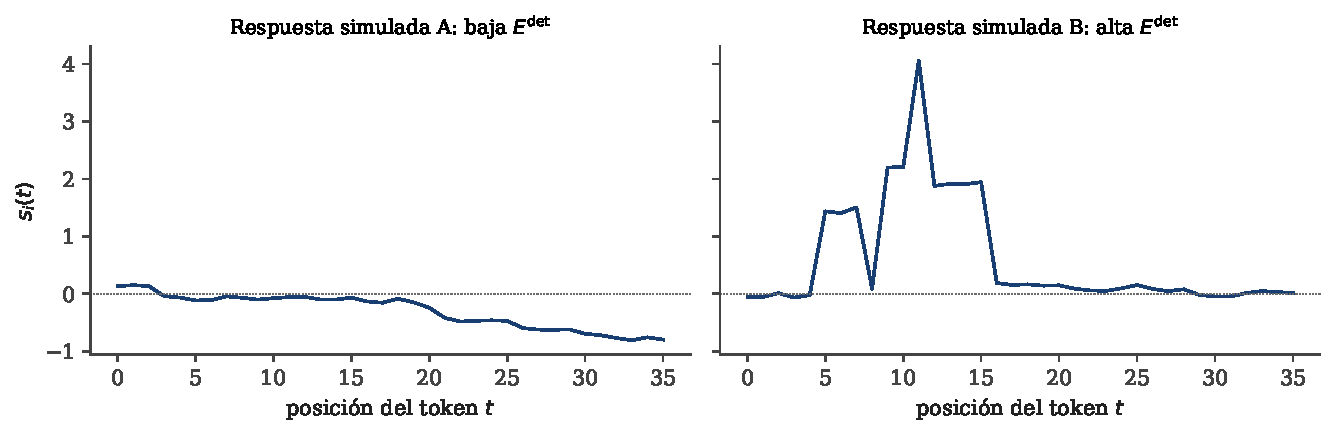
\includegraphics[width=0.92\linewidth]{figs/fig_señal_ejemplo.pdf}
\caption{Dos señales posicionales simuladas $s_i(t)$: una con baja intensidad emocional
impuesta (izquierda) y otra con ráfagas locales marcadas (derecha), que producen
$E^{\mathrm{det}}$ bajo y alto respectivamente.}
\label{fig:señal}
\end{figure}

\begin{figure}[htb]
\centering
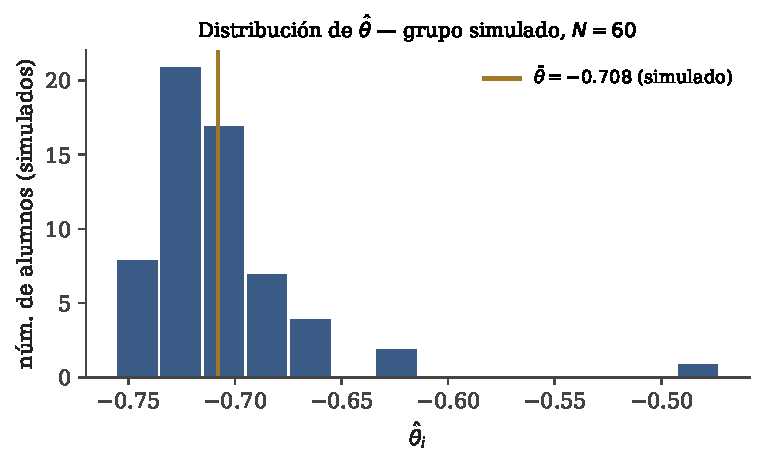
\includegraphics[width=0.75\linewidth]{figs/fig_theta_hist.pdf}
\caption{Distribución de $\hat\theta$ sobre el grupo simulado ($N=60$). La asimetría visible es
consistente con el rechazo de normalidad reportado en el texto (Shapiro--Wilk $p<10^{-3}$).}
\label{fig:theta_hist}
\end{figure}

\begin{figure}[htb]
\centering
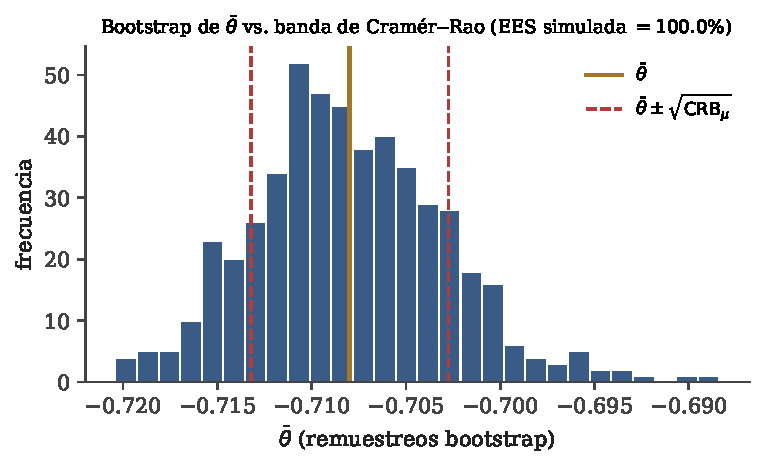
\includegraphics[width=0.75\linewidth]{figs/fig_bootstrap_crb.pdf}
\caption{Distribución bootstrap de $\bar\theta$ ($B=500$) contra la banda
$\bar\theta\pm\sqrt{\mathrm{CRB}_\mu}$. En esta simulación $\mathrm{EES}=100\%$
\emph{a pesar de} que $\hat\theta$ rechaza normalidad — el punto central de la
\cref{sec:crb}: esta cifra no mide si el pipeline extrae información del texto.}
\label{fig:bootstrap}
\end{figure}

\begin{figure}[htb]
\centering
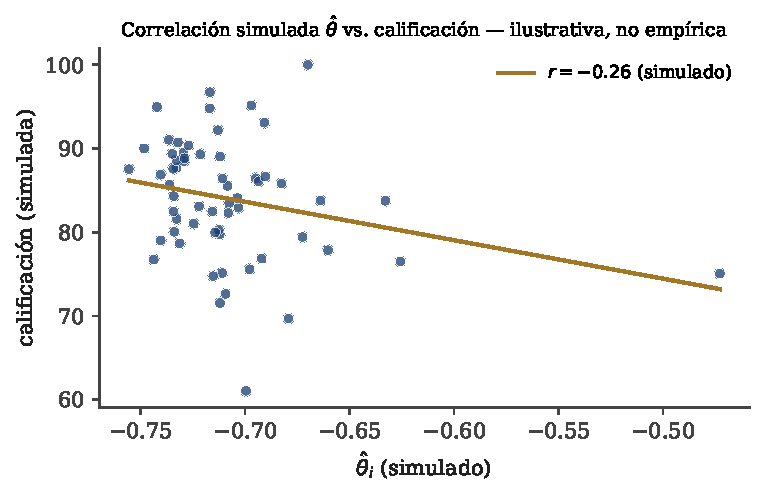
\includegraphics[width=0.75\linewidth]{figs/fig_correlacion.pdf}
\caption{Correlación simulada entre $\hat\theta$ y la calificación, impuesta por construcción
($c_i$ se definió como función decreciente de la intensidad emocional simulada $e_i$) para
ilustrar cómo se lee esta gráfica en la interfaz real.}
\label{fig:correlacion}
\end{figure}

\FloatBarrier

\section{Discusión y limitaciones}

El sistema es una herramienta de apoyo a la decisión docente, no un instrumento diagnóstico
automatizado. El índice $\hat\theta$ depende del modelo de embeddings elegido, de la familia y
nivel de la wavelet, y del tamaño de la encuesta; con $N<30$ las estimaciones bootstrap de
varianza son inestables y el propio sistema advierte de ello en la interfaz. Las
interpretaciones textuales que genera el módulo \texttt{interpretacion.py} son sugerencias de
lectura, no conclusiones definitivas, y deben cotejarse con el criterio del docente y, cuando
el caso lo amerite, con apoyo psicopedagógico institucional. Como se documentó en
\cref{sec:crb}, la verificación de Cramér--Rao certifica la coherencia estadística de
$\bar\theta$ bajo el modelo supuesto, no la calidad de $\hat\theta$ como medida de sentimiento;
esa segunda pregunta —la que de verdad importaría validar— queda abierta y requeriría
comparación externa (anotación humana, u otra pipeline de extracción) sobre datos reales de
curso, algo que este artículo deliberadamente no reporta.

\begin{implBox}
Interfaz Streamlit (\texttt{app.py}) con cuatro páginas modulares
(\texttt{pages/carga.py}, \texttt{pages/metricas.py}, \texttt{pages/sentimiento.py},
\texttt{pages/validacion.py}); \texttt{sentence-transformers} para embeddings,
\texttt{PyWavelets} para la DWT, \texttt{scipy.stats} para Shapiro--Wilk y correlación de
Pearson, \texttt{plotly} para visualización interactiva (incluyendo histograma bootstrap de
$\bar\theta$ con bandas $\pm\sqrt{\mathrm{CRB}}$, comparación de varianzas, y gráfica Q--Q de
$\hat\theta$ contra la normal). Código y datos de ejemplo en
\href{https://github.com/Gabriel44svg/Galindo-C.-J.-y-Villafuerte-C.-G.-2026-.-SIAMDA}{github.com/Gabriel44svg/Galindo-C.-J.-y-Villafuerte-C.-G.-2026-.-SIAMDA}.
\end{implBox}

\section{Conclusión}

Este sistema integra dos señales de un curso —calificaciones y respuestas abiertas de
encuesta— bajo un mismo tablero, y añade a la segunda una métrica reproducible ($\hat\theta$,
vía embeddings de token, proyección posicional y DWT) junto con una verificación estadística de
la coherencia de su media agregada (información de Fisher y cota de Cramér--Rao, bajo modelos
gaussiano y Laplaciano). El resultado es un sistema de alerta temprana que hace explícito, en
vez de impresionista, el vínculo entre el tono de las respuestas de un grupo y su desempeño, y
que documenta honestamente qué certifica su capa estadística y qué no. Queda como trabajo futuro
la validación de $\hat\theta$ contra anotación humana sobre datos reales de curso.

\begin{thebibliography}{9}

\bibitem{Fisher1922} R.~A.~Fisher, \emph{On the mathematical foundations of theoretical
statistics}, Philos. Trans. R. Soc. Lond. A \textbf{222} (1922), 309--368.

\bibitem{Rao1945} C.~R.~Rao, \emph{Information and the accuracy attainable in the estimation of
statistical parameters}, Bull. Calcutta Math. Soc. \textbf{37} (1945), 81--91.

\bibitem{Cramer1946} H.~Cram\'er, \emph{Mathematical Methods of Statistics}, Princeton University
Press, 1946.

\bibitem{ShapiroWilk1965} S.~S.~Shapiro and M.~B.~Wilk, \emph{An analysis of variance test for
normality (complete samples)}, Biometrika \textbf{52} (1965), no.~3/4, 591--611.

\bibitem{Efron1979} B.~Efron, \emph{Bootstrap methods: another look at the jackknife}, Ann.
Statist. \textbf{7} (1979), no.~1, 1--26.

\bibitem{Pearson1896} K.~Pearson, \emph{Mathematical contributions to the theory of evolution.
III. Regression, heredity, and panmixia}, Philos. Trans. R. Soc. Lond. A \textbf{187} (1896),
253--318.

\bibitem{Mallat1989} S.~G.~Mallat, \emph{A theory for multiresolution signal decomposition: the
wavelet representation}, IEEE Trans. Pattern Anal. Mach. Intell. \textbf{11} (1989), no.~7,
674--693.

\bibitem{ReimersGurevych2019} N.~Reimers and I.~Gurevych, \emph{Sentence-BERT: sentence
embeddings using Siamese BERT-networks}, in Proc.\ 2019 Conf.\ Empirical Methods in Natural
Language Processing (EMNLP-IJCNLP), Hong Kong, 2019, pp.~3982--3992.

\end{thebibliography}

\end{document}
